% ★★ 中档
\newcommand{\qConicDefTwoDerivationStem}{
平面内任意一点 $P(x,y)$ 到点 $F(c, 0)$ 的距离与到定直线 $l: x = \frac{a^2}{c}$ 的距离之比为常数 $e$（其中 $a > c > 0$），且 $e = \frac{c}{a}$．求点 $P$ 的轨迹方程，并对 $0 < e < 1$ 和 $e > 1$ 的两种情况分别进行讨论与化简．
}
\newcommand{\qConicDefTwoDerivationFigure}{
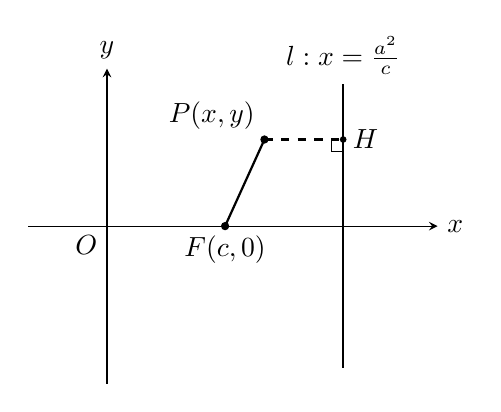
\begin{tikzpicture}[scale=1, >=stealth]
  % Axes
  \draw[->] (-1,0) -- (4.2,0) node[right] {$x$};
  \draw[->] (0,-2) -- (0,2) node[above] {$y$};
  \node[below left] at (0,0) {$O$};
  
  % Focus F
  \coordinate (F) at (1.5,0);
  \fill (F) circle (1.5pt);
  \node[below] at (F) {$F(c,0)$};
  
  % Directrix l
  \draw[thick] (3, -1.8) -- (3, 1.8);
  \node[above] at (3, 1.8) {$l: x=\frac{a^2}{c}$};
  
  % Point P
  \coordinate (P) at (2, 1.1);
  \fill (P) circle (1.5pt);
  \node[above left] at (P) {$P(x,y)$};
  
  % H on directrix
  \coordinate (H) at (3, 1.1);
  \fill (H) circle (1.2pt);
  \node[right] at (H) {$H$};
  
  % Lines
  \draw[thick] (P) -- (F);
  \draw[thick, dashed] (P) -- (H);
  
  % Right angle at H
  \draw (2.85, 1.1) -- (2.85, 0.95) -- (3, 0.95);
\end{tikzpicture}
}
\newcommand{\qConicDefTwoDerivationAnswer}{
当 $0 < e < 1$ 时，轨迹为焦点在 $x$ 轴的椭圆：$\frac{x^2}{a^2} + \frac{y^2}{b^2} = 1$（其中 $b^2 = a^2 - c^2$）；当 $e > 1$ 时，轨迹为焦点在 $x$ 轴的双曲线：$\frac{x^2}{a^2} - \frac{y^2}{b^2} = 1$（其中 $b^2 = c^2 - a^2$）．
}
\newcommand{\qConicDefTwoDerivationSolution}{
由题意，点 $P(x,y)$ 满足：
\[
\frac{PF}{d(P,l)} = e \implies \frac{\sqrt{(x-c)^2+y^2}}{\left|x-\frac{a^2}{c}\right|} = e
\]
将分母乘到等式右边，两边平方得：
\[
(x-c)^2 + y^2 = e^2 \left(x - \frac{a^2}{c}\right)^2
\]
由于 $e = \frac{c}{a}$，代入上式得：
\[
(x-c)^2 + y^2 = \frac{c^2}{a^2} \left(x - \frac{a^2}{c}\right)^2
\]
展开整理得：
\[
x^2 - 2cx + c^2 + y^2 = \frac{c^2}{a^2} \left(x^2 - \frac{2a^2}{c}x + \frac{a^4}{c^2}\right)
\]
\[
x^2 - 2cx + c^2 + y^2 = \frac{c^2}{a^2}x^2 - 2cx + a^2
\]
消去两边的 $-2cx$，并将含 $x, y$ 的项移到等式左边，常数项移到等式右边得：
\[
\left(1 - \frac{c^2}{a^2}\right)x^2 + y^2 = a^2 - c^2 \implies \frac{a^2 - c^2}{a^2}x^2 + y^2 = a^2 - c^2
\]
由于 $a > c > 0$，所以 $a^2 - c^2 \neq 0$，两边同除以 $a^2 - c^2$ 得：
\[
\frac{x^2}{a^2} + \frac{y^2}{a^2 - c^2} = 1
\]
下面对 $e$ 的取值进行讨论：
\begin{enumerate}[label=\arabic*.]
  \item 当 $0 < e < 1$ 时，由 $e = \frac{c}{a}$ 得 $c < a$，即 $a^2 - c^2 > 0$．\\
  令 $b^2 = a^2 - c^2\ (b > 0)$，则方程化为：
  \[
  \frac{x^2}{a^2} + \frac{y^2}{b^2} = 1
  \]
  此时轨迹为焦点在 $x$ 轴上的椭圆．
  \item 当 $e > 1$ 时，由 $e = \frac{c}{a}$ 得 $c > a$，即 $a^2 - c^2 < 0$，此时 $c^2 - a^2 > 0$．\\
  令 $b^2 = c^2 - a^2\ (b > 0)$，即 $a^2 - c^2 = -b^2$，则方程化为：
  \[
  \frac{x^2}{a^2} - \frac{y^2}{b^2} = 1
  \]
  此时轨迹为焦点在 $x$ 轴上的双曲线．
\end{enumerate}
}
\newcommand{\qConicDefTwoDerivationDiagnosis}{
\errortag{平方根式化简错误} 学生在去绝对值和去根式进行平方展开时，容易在交叉项（如 $-2cx$）的消去上出现计算失误．\\
\errortag{离心率范围讨论缺失} 部分学生仅能推导至最终方程形式，但忽视了当 $e>1$ 时 $a^2-c^2 < 0$ 的符号判定，导致无法正确化简出双曲线标准方程的负号．
}
